% Wasserstein GAN - April 2017
% Nishant D. Gurnani

\documentclass{beamer}
\mode<presentation> {
\usetheme{default}
\setbeamertemplate{footline}[page number]
\setbeamercovered{invisible}
% To remove the navigation symbols from the bottom of slides%
\setbeamertemplate{navigation symbols}{} 
}

\usepackage{mathtools}
\DeclarePairedDelimiter{\ceil}{\lceil}{\rceil}

\newcounter{saveenumi}
\newcommand{\seti}{\setcounter{saveenumi}{\value{enumi}}}
\newcommand{\conti}{\setcounter{enumi}{\value{saveenumi}}}


\newcommand{\id}{\mathrm{id}}
\newcommand{\K}{\mathrm{KL}}
\newcommand{\kl}{\mathrm{kl}}
\newcommand{\bp}{\boldsymbol{p}}
\renewcommand{\phi}{\varphi}
\renewcommand{\a}{\alpha}

\renewcommand{\P}{\mathbb{P}}
\newcommand{\E}{\mathbb{E}}
\newcommand{\N}{\mathbb{N}}
\newcommand{\R}{\mathbb{R}}
\newcommand{\Q}{\mathbb{Q}}
\newcommand{\KL}{\mathrm{KL}}
\newcommand{\LG}{\overline{\log}(d)}
\newcommand{\LGG}{\overline{\log}(M K)}
\newcommand{\ocP}{\overline{\mathcal{P}}}

\newcommand{\cO}{\mathcal{O}}
\newcommand{\cZ}{\mathcal{Z}}
\newcommand{\cA}{\mathcal{A}}
\newcommand{\cB}{\mathcal{B}}
\newcommand{\cN}{\mathcal{N}}
\newcommand{\cM}{\mathcal{M}}
\newcommand{\cF}{\mathcal{F}}
\newcommand{\cL}{\mathcal{L}}
\newcommand{\cX}{\mathcal{X}}
\newcommand{\cI}{\mathcal{I}}
\newcommand{\cJ}{\mathcal{J}}
\newcommand{\cY}{\mathcal{Y}}
\newcommand{\cH}{\mathcal{H}}
\newcommand{\cP}{\mathcal{P}}
\newcommand{\cT}{\mathcal{T}}
\newcommand{\cC}{\mathcal{C}}
\newcommand{\cS}{\mathcal{S}}
\newcommand{\cE}{\mathcal{E}}
\newcommand{\cK}{\mathcal{K}}
\newcommand{\cD}{\mathcal{D}}

\newcommand{\oD}{\overline{\mathcal{D}}}
\newcommand{\oR}{\overline{R}}

\def\ds1{\mathds{1}}
\renewcommand{\epsilon}{\varepsilon}

\newcommand{\wh}{\widehat}
\newcommand{\argmax}{\mathop{\mathrm{argmax}}}
\newcommand{\argmin}{\mathop{\mathrm{argmin}}}
\renewcommand{\mod}[2]{[#1 \,\, \mathrm{mod} \,\, #2]}
\newcommand{\todo}{{\bf TO DO } }

\renewcommand{\tilde}{\widetilde}

%Cadres d'algorithmes
\newlength{\minipagewidth}
\setlength{\minipagewidth}{\columnwidth}
\setlength{\fboxsep}{3mm}
\addtolength{\minipagewidth}{-\fboxrule}
\addtolength{\minipagewidth}{-\fboxrule}
\addtolength{\minipagewidth}{-\fboxsep}
\addtolength{\minipagewidth}{-\fboxsep}
\newcommand{\bookbox}[1]{\small
\par\medskip\noindent
\framebox[\columnwidth]{
\begin{minipage}{\minipagewidth} {#1} \end{minipage} } \par\medskip }

%%
%

\newcommand{\Ber}{\mathop{\mathrm{Ber}}}

\newcommand{\beq}{\begin{equation}}
\newcommand{\eeq}{\end{equation}}

\newcommand{\beqa}{\begin{eqnarray}}
\newcommand{\eeqa}{\end{eqnarray}}

\newcommand{\beqan}{\begin{eqnarray*}}
\newcommand{\eeqan}{\end{eqnarray*}}

\def\ba#1\ea{\begin{align*}#1\end{align*}} %\ba = \begin{algin*}, \ea = \end{align*}
\def\banum#1\eanum{\begin{align}#1\end{align}} %\banum = \begin{algin}, \eanum

%\newcommand{\qed}{\hfill\BlackBox}
\newcommand{\charfct}{\ds1} %
\newcommand{\Fcal}{\mathcal{F}}
\newcommand{\Xcal}{\mathcal{X}}
\newcommand{\Hcal}{\mathcal{H}}
\newcommand{\Gcal}{\mathcal{G}}
\newcommand{\Nat}{\mathbb{N}}


% For citations
\usepackage{natbib}

\usepackage{graphicx}
\usepackage{subfig}
\usepackage{bm} 


\newcounter{saveenumi}
\newcommand{\seti}{\setcounter{saveenumi}{\value{enumi}}}
\newcommand{\conti}{\setcounter{enumi}{\value{saveenumi}}}

\resetcounteronoverlays{saveenumi}

%\setbeamerfont{institute}{size=\medium}
\setbeamerfont{date}{size=\tiny}


\title[]{A Case Study on Volatility in Financial Time Series}
%
\author{Nishant Gurnani}
\date{June 4th, 2018}

\begin{document}

% Title Slide
\begin{frame}
\titlepage
\end{frame}


% TOC SLIDE --> NEED TO FIX!!
\begin{frame}
\frametitle{Outline}
\tableofcontents
\end{frame}

\section{What is Volatility?}
%% INTRODUCTION
\begin{frame}
\frametitle{Outline}
\tableofcontents[currentsection]
\end{frame}

\section{Exploratory Data Analysis with NoVaS}
\section{Predicting $Y_{t}^2$ as a proxy for Volatility}
\section{A simple Volatility trading strategy}





% MOTIVATION SLIDE
\begin{frame}
\frametitle{Why are these Papers Important?}
\begin{itemize}

\pause
\vspace{-20pt}
\item{Recently a large number of GAN frameworks have been proposed - BGAN, LSGAN, DCGAN, DiscoGAN $\dots$}
\pause
\item{Wasserstein GAN is yet another GAN training algorithm, however it is backed up by rigorous theory in addition to good performance}
\pause
\item{WGAN removes the need to balance generator updates with discriminator updates, thus removing a key source of training instability in the original GAN}
\pause
\item{Empirical results show correlation between discriminator loss and perceptual quality thus providing a rough measure of training progress}
\end{itemize}
\pause
\vspace{10pt}
\textbf{Goal - \textcolor{red} {Convince you that WGAN is the ``best" GAN}}
\end{frame}



\begin{frame}
\frametitle{What does it mean to learn a probability distribution?}

\vspace{-20pt}

When learning generative models, we assume the data we have comes from some unknown distribution $\P_{r}$. \\ \vspace{10pt}

Want to learn a distribution $\P_{\theta}$ that approximates $\P_{r}$, where $\theta$ are the parameters of the distribution.

\vspace{10pt}

There are two approaches for doing this:
\pause
\begin{enumerate}
\item{Directly learn the probability density function $\P_{\theta}$ and then optimize through maximum likelihood estimation}
\vspace{5pt}
\pause
\item{Learn a function that transforms an existing distribution $Z$ into $\P_{\theta}$. Here, $g_{\theta}$ is some differentiable function, $Z$ is a common distribution (usually uniform or Gaussian), and $\P_{\theta} = g_{\theta}(Z)$}
\end{enumerate}
\end{frame}

\begin{frame}
\frametitle{Maximum Likelihood approach is problematic}
\vspace{5pt}
Recall that for continuous distributions $\P$ and $\Q$ the $KL$ divergence is:
\vspace{-2.5pt}
$$ KL(\P||\Q) = \int_{x} \P(x) \log\frac{\P(x)}{\Q(x)} dx $$

and given function $\P_{\theta}$, the MLE objective is 

$$ \max_{\theta \in \R^d} \frac{1}{m} \sum_{i=1}^{m} \log \P_{\theta}(x^{(i)}) $$
\vspace{5pt}
In the limit (as $m \to \infty$), samples will appear based on the data distribution $\P_{r}$, so
\vspace{-2.5pt}
\begin{align*}
\lim_{m \to \infty} \max_{\theta \in \R^d} \frac{1}{m} \sum_{i=1}^{m} \log \P_{\theta}(x^{(i)}) &= \max_{\theta \in \R^d} \int_{x} \P_{r}(x) \log \P_{\theta}(x) dx \\
\end{align*}
\end{frame}


\begin{frame}
\frametitle{Maximum Likelihood approach is problematic}
\vspace{-15pt}
\begin{align*}
\lim_{m \to \infty} \max_{\theta \in \R^d} \frac{1}{m} \sum_{i=1}^{m} \log \P_{\theta}(x^{(i)}) &= \max_{\theta \in \R^d} \int_{x} \P_{r}(x) \log \P_{\theta}(x) dx \\
&= \min_{\theta \in \R^d} - \int_{x} \P_{r}(x) \log \P_{\theta}(x) dx \\
&= \min_{\theta \in \R^d} \int_{x} \P_{r}(x) \log \P_{r}(x) dx - \int_{x} \P_{r}(x) \log \P_{\theta}(x) dx \\
&= \min_{\theta \in \R^d} KL(\P_{r}||\P_{\theta})
\end{align*}

\begin{itemize}
\pause
\item{Note if $\P_{\theta} = 0$ at an $x$ where $\P_{r} > 0$, the $KL$ divergence goes to $+\infty$ (bad for the MLE if $\P_{\theta}$ has low dimensional support)}
\vspace{2.5pt}
\pause
\item{Typical remedy is to add a noise term to the model distribution to ensure distribution is defined everywhere}
\vspace{2.5pt}
\pause
\item{This unfortunately introduces some error, and empirically people have needed to add a lot of random noise to make models train}
\end{itemize}
\end{frame}

\begin{frame}
\frametitle{Transforming an existing distribution}

Shortcomings of the maximum likelihood approach motivate the second approach of learning a $g_{\theta}$ (a generator) to transform a known distribution Z.
\vspace{5pt}

Advantages of this approach:
\pause
\begin{itemize}
\item{Unlike densities, this approach can represent distributions confined to a low dimensional manifold}
\pause
\item{It's very easy to generate samples - given a trained $g_{\theta}$, simply sample random noise $z \sim Z$, and evaluate $g_{\theta}(z)$}
\end{itemize}
\pause
\begin{block} {VAEs and GANs are well known examples of this approach}
VAEs focus on the approximate likelihood of the examples and so share the limitation that you need to fiddle with additional noise terms. \\
\vspace{2.5pt}
\pause
GANs offer much more flexibility but their training is unstable.
\end{block}
\end{frame}


\begin{frame}
\frametitle{Transforming an existing distribution}

To train $g_{\theta}$ (and by extension $\P_{\theta}$), we need a measure of distance between distributions i.e. $d(\P_{r},\P_{\theta})$.
\pause
\begin{block}{Distance Properties}
\begin{itemize}
\pause
\item{Distance $d$ is weaker than distance $d'$ if every sequence that converges under $d'$ converges under $d$}
\pause
\item{Given a distance $d$, we can treat $d(\P_{r},\P_{\theta})$ as a loss function}
\pause
\item{We can minimize $d(\P_{r},\P_{\theta})$ with respect to $\theta$ as long as the mapping $\theta \mapsto \P_{\theta}$ is continuous (true if $g_{\theta}$ is a neural network)}

\end{itemize}
\end{block}
\pause
\begin{center}
\textcolor{red}{\textbf{How do we define $d$?}}
\end{center}

\end{frame}

% Different Distances
\section{Different Distances}

\begin{frame}
\tableofcontents[currentsection]
\end{frame}

\begin{frame}
\frametitle{Distance definitions}

\pause
\begin{block}{Notation}
$\chi$ - compact metric set (such as the space of images $[0,1]^d$)\\
$\Sigma$ - set of all Borel subsets of $\chi$ \\
Prob($\chi$) - space of probability measures defined on $\chi$\\
\end{block}

%We can now define elementary distances and divergences between two distributions $\P_{r}, \P_{\theta} \in$ Prob($\chi$).
\pause
\begin{block}{Total Variation (TV) distance}
\vspace{-5pt}
$$ \delta(\P_{r}, \P_{\theta}) = \sup_{A \in \Sigma} |\P_{r}(A) - \P_{\theta} (A)| $$
\vspace{-5pt}
\end{block}
\pause
\begin{block}{Kullback-Leibler (KL) divergence}
\vspace{-5pt}
$$ KL(\P_{r}||\P_{\theta}) = \int_{x} \P_{r}(x) \log\frac{\P_{r}(x)}{\P_{\theta}(x)} d\mu(x) $$

where both $\P_{r}$ and $\P_{\theta}$ are assumed to be absolutely continuous with respect to a same measure $\mu$ defined on $\chi$. 

\end{block}

\end{frame}

\begin{frame}
\frametitle{Distance Definitions}

\pause
\begin{block}{Jensen-Shannon (JS) Divergence}

$$ JS(\P_{r}, \P_{\theta}) = KL(\P_{r}||\P_{m}) + KL(\P_{\theta}||\P_{m}) $$

where $\P_{m}$ is the mixture $(\P_{r} + \P_{\theta})/2$ 
\end{block}
\pause
\begin{block}{Earth-Mover (EM) distance or Wasserstein-1}

$$ W(\P_{r},\P_{\theta}) = \inf_{\gamma \in \Pi((\P_{r},\P_{\theta})} \E_{(x,y) \sim \gamma} [ ||x-y|| ] $$

where $\Pi(\P_{r},\P_{\theta})$ denotes the set of all join distributions $\gamma(x,y)$ whose marginals are respectively $\P_{r}$ and $\P_{\theta}$\\
\vspace{2.5pt}
%$\gamma(x,y)$ indicates how much ``mass" must be transported from $x$ to $y$ in order to transform the distribution $\P_{r}$ into the distribution $\P_{\theta}$\\
%\vspace{2.5pt}
%The EM distance then is the ``cost" of the optimal transport plan
\end{block}

\end{frame}


\begin{frame}
\frametitle{Understanding the EM distance}
\pause
\begin{block}{Main Idea}
Probability distributions are defined by how much mass they put on each point. \\
\vspace{0.12in}
\pause
Imagine we started with distribution $\P_{r}$, and wanted to move mass around to change the distribution into $\P_{\theta}$. \\
\vspace{0.12in}
\pause
Moving mass $m$ by distance $d$ costs $m \cdot d$ effort. \\
\vspace{0.12in}
\pause
The earth mover distance is the minimal effort we need to spend. \\
\end{block}
\pause
\begin{block}{Transport Plan}
Each $\gamma \in \Pi$ is a transport plan and to execute the plan, for all $x,y$ move $\gamma(x,y)$ mass from $x$ to $y$.

\end{block}
\end{frame}

\begin{frame}
\frametitle{Understanding the EM distance}

\pause
What properties does the plan need to satisfy to transform $\P_{r}$ into $\P_{\theta}$? \\
\vspace{0.12in}
\pause
The amount of mass that leaves $x$ is $\int_{y} \gamma(x,y) dy$. This must equal $\P_{r}(x)$, the amount of mass originally at $x$.\\
\vspace{0.12in}
\pause
The amount of mass that enters $y$ is $\int_{x} \gamma(x,y) dx$. This must equal $\P_{\theta}(y)$, the amount of mass that ends up at y.\\
\vspace{0.12in}
\pause
This shows why the marginals of $\gamma \in \Pi$ must be $\P_{r}$ and $\P_{\theta}$. For scoring, the effort spent is $$\int_{x} \int_{y} \gamma(x,y) ||x-y|| dydx = \E_{(x,y) \sim \gamma} [ ||x-y|| ]$$\\
\vspace{0.12in}
\pause
Computing the infimum of this over all valid $\gamma$ gives the earth mover distance
\end{frame}


\begin{frame}
\frametitle{Learning Parallel Lines Example}
\pause
Let $Z \sim U[0,1]$ and let $\P_{0}$ be the distribution of $(0,Z) \in \R^2$, uniform on a straight vertical line passing through the origin. Now let $g_{\theta}(z) = (\theta,z)$ with $\theta$ a single real parameter.
\pause
\begin{figure}
\centering
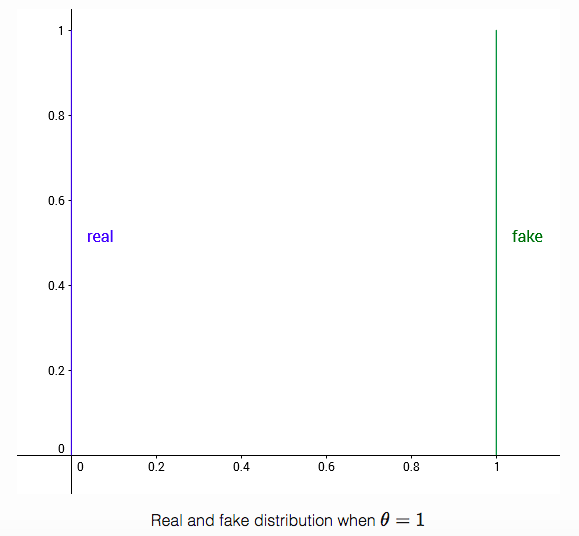
\includegraphics[width=0.5\textwidth]{parallel_lines.png}
\end{figure}

\pause
We'd like our optimization algorithm to learn to move $\theta$ to $0$. As $\theta \to 0$, the distance $d(\P_{0},\P_{\theta})$ should decrease.

\end{frame}

\begin{frame}
\frametitle{Learning Parallel Lines Example}
For many common distance functions, this doesn't happen.
\pause
\begin{equation*}
\delta(\P_{0},\P_{\theta}) = \begin{cases}
1 &\text{if $\theta \neq 0$}\\    
0 &\text{if $\theta = 0$}
\end{cases}
\end{equation*}

\begin{equation*}
JS(\P_{0},\P_{\theta}) = \begin{cases}
\log 2 &\text{if $\theta \neq 0$}\\    
0 &\text{if $\theta = 0$}
\end{cases}
\end{equation*}

\begin{equation*}
KL(\P_{\theta}, \P_{0}) = KL(\P_{0},\P_{\theta}) = \begin{cases}
+\infty &\text{if $\theta \neq 0$}\\    
0 &\text{if $\theta = 0$}
\end{cases}
\end{equation*}

$$W(\P_{0},\P_{\theta}) = |\theta|$$

\end{frame}

\begin{frame}
\frametitle{Theoretical Justification}
\begin{Theorem}[1]
Let $\P_{r}$ be a fixed distribution over $\chi$. Let $Z$ be a random variable over another space $\mathcal{Z}$. Let $g: \mathcal{Z} \times \R^{d} \to \chi$ be a function, that will be denote $g_{\theta}(z)$ with $z$ the first coordinate and $\theta$ the second. Let $\P_{\theta}$ denote the distribution of $g_{\theta}(\Z)$. Then,
\begin{enumerate}
\item{If $g$ is continuous in $\theta$, so is $W(\P_{r},\P_{\theta})$.}
\item{If $g$ is locally Lipschitz and satisfies regularity assumption 1, then $W(\P_{r},\P_{\theta})$ is continuous everywhere, and differentiable almost everywhere}
\item{Statements 1-2 are false for the Jensen-Shannon divergence $JS(\P_{r}, \P_{\theta})$ and all the KLs.}
\end{enumerate}
\end{Theorem}
\end{frame}

\begin{frame}
\frametitle{Theoretical Justification}

%\begin{Corollary}
%Let $g_{\theta}$ be any feedforward neural network parametrized by $\theta$, and a prior over $z$ such that $\E_{z \sim p(z)}[|z|] < \infty$ (e.g. Gaussian, uniform etc.) Then assumption 1 is satisfied and therefore $W(\P_{r},\P_{\theta})$ is continuous everywhere and differentiable almost everywhere.
%\end{Corollary}


\begin{Theorem}[2]
Let $\P$ be a distribution on a compact space $\chi$ and $(\P_{n})_{n \in \N}$ be a sequence of distributions on $\chi$. Then, considering all limits as $n \to \infty$,
\begin{enumerate}
\item{The following statements are equivalent
\begin{itemize}
\item{$\delta(\P_{n}, \P) \to 0$}
\item{$JS(\P_{n}, \P) \to 0$}
\end{itemize}
}
\item{The following statements are equivalent
\begin{itemize}
\item{$W(\P_{n}, \P) \to 0$}
\item{$\P_{n} \overset{D}{\to} \P$ where $\overset{D}{\to}$ represents convergence in distribution for random variables}
\end{itemize}
}
\item{$KL(\P_{n}||\P) \to 0$ or $KL(\P||\P_{n}) \to 0$ imply the statements in (1).}
\item{The statements in (1) imply the statements in (2).}
\end{enumerate}
\end{Theorem}
\end{frame}

% Standard GAN
\section{Standard GAN}
\begin{frame}
\tableofcontents[currentsection]
\end{frame}

\begin{frame}
\frametitle{Generative Adversarial Networks}

Recall that the GAN training strategy is to define a game between two competing networks.\\
\vspace{15pt}
\pause
The $generator$ network $G$ maps a source of noise to the input space. \\
\vspace{15pt}
\pause
The $discriminator$ network $D$ receives either a generated sample or a true data sample and must distinguish between the two.\\
\vspace{15pt}
\pause
The generator is trained to fool the discriminator.\\
\vspace{15pt}
\end{frame}


\begin{frame}
\frametitle{Generative Adversarial Networks}
\vspace{-0.6in}
Formally we can express the game between the generator $G$ and the discriminator $D$ with the minimax objective:
\vspace{0.2in}
$$ \min_{G} \max_{D} \E_{x \sim \P_{r}} [\log(D(x))] + \E_{\tilde{x} \sim \P_{g}} [\log(1 - D(\tilde{x})] $$
where $\P_{r}$ is the data distribution and $\P_{g}$ is the model distribution implicitly defined by $\tilde{x} = G(z)$, $z \sim p(z)$

\end{frame}


\begin{frame}
\frametitle{Generative Adversarial Networks}

\begin{block}{Remarks}
\begin{itemize}
\pause
\item{If the discriminator is trained to optimality before each generator parameter update, minimizing the value function amounts to minimizing the Jensen-Shannon divergence between the data and model distributions on $x$}
\pause
\item{This is expensive and often leads to vanishing gradients as the discriminator saturates}
\pause
\item{In practice, this requirement is relaxed, and the generator and discriminator are update simultaneously}
\end{itemize}
\end{block}


\end{frame}


\section{Wasserstein GAN}
\begin{frame}
\tableofcontents[currentsection]
\end{frame}

\begin{frame}
\frametitle{Kantorivich-Rubinstein Duality}
Unfortunately, computing the Wasserstein distance exactly is intractable.

$$ W(\P_{r},\P_{\theta}) = \inf_{\gamma \in \Pi((\P_{r},\P_{\theta})} \E_{(x,y) \sim \gamma} [ ||x-y|| ] $$

\pause
However, a result from the Kantorivich-Rubinstein Duality (Villani 2008)  shows $W$ is equivalent to

$$ W(\P_{r},\P_{\theta}) = \sup_{||f||_{L} \leq 1} \E_{x \sim \P_{r}}[f(x)] - \E_{x \sim \P_{\theta}}[f(x)] $$

where the supremum is taken over all 1-Lipschitz functions\\ \vspace{0.2in}
\pause
\textbf{Calculating this is still intractable, but now it's easier to approximate.}

\end{frame}

\begin{frame}
\frametitle{Wasserstein GAN Approximation}
\pause
Note that if we replace the supremum over 1-Lipschitz functions with the supremum over $K$-Lipschitz functions, then the supremum is $K \cdot W(\P_{r},\P_{\theta})$ instead.\\
\pause
\vspace{0.12in}
Suppose we have a parametrized function family $\{f_{w}\}_{w \in W}$, where $w$ are the weights and $W$ is the set of all possible weights\\
\vspace{0.12in}
Furthermore suppose these functions are all $K$-Lipschitz for some $K$. \pause Then we have
\vspace{-0.07in}
$$\max_{w \in W} \E_{x \sim \P_{r}}[f_{w}(x)] - \E_{x \sim \P_{\theta}}[f_{w}(x)] \leq \sup_{||f||_{L} \leq K} \E_{x \sim \P_{r}}[f(x)] - \E_{x \sim \P_{\theta}}[f(x)]$$
$$ \hspace{1in}= K \cdot W(\P_{r},\P_{\theta})$$
\pause
If $\{f_{w}\}_{w \in W}$ contains the true supremum among $K$-Lipschitz functions, this gives the distance exactly.\\
\vspace{0.1in}
\pause
\textbf{In practice this won't be true!}


\end{frame}

\begin{frame}
\frametitle{Wasserstein GAN Algorithm}

Looping all this back to generative models, we'd like to train $\P_{\theta} = g_{\theta}(z)$ to match $\P_{r}$.\\
\vspace{0.12in}
\pause
Intuitively, given a fixed $g_{\theta}$, we can compute the optimal $f_{w}$ for the Wasserstein distance.\\
\pause
\vspace{0.12in}
We can then backpropagate through $W(\P_{r},g_{\theta}(Z))$ to get the gradient for $\theta$.

$$ \nabla_{\theta} W(\P_{r},\P_{\theta}) = \nabla_{\theta}(\E_{x \sim \P_{r}}[f_{w}(x)] - \E_{z\sim Z}[f_{w}(g_{\theta}(z))]) $$
$$ \hspace{-0.08in}= -\E_{z\sim Z}[\nabla_{\theta} f_{w}(g_{\theta}(z))] $$

\end{frame}


\begin{frame}
\frametitle{Wasserstein GAN Algorithm}
The training process now has three steps:
\begin{enumerate}
\pause
\item{For a fixed $\theta$, compute an approximation of $W(\P_{r},\P_{\theta})$ by training $f_{w}$ to convergence}
\pause
\item{Once we have the optimal $f_{w}$, compute the $\theta$ gradient $-\E_{z\sim Z}[\nabla_{\theta} f_{w}(g_{\theta}(z))]$ by sampling several $z \sim Z$}
\pause
\item{Update $\theta$, and repeat the process}
\end{enumerate}
\pause
\begin{block}{Important Detail}
The entire derivation only works when the function family $\{f_{w}\}_{w \in W}$ is $K$-Lipschitz.\\
\vspace{0.12in}
\pause
To guarantee this is true, the authors use weight clamping. The weights $w$ are constrained to lie within $[-c,c]$, by clipping $w$ after every update to $w$.\\
\end{block}
\end{frame}

\begin{frame}
\frametitle{Wasserstein GAN Algorithm}
\begin{figure}
\centering
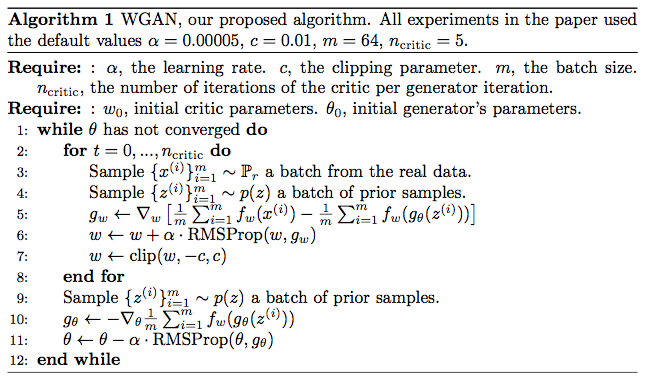
\includegraphics[width=1.07\textwidth]{wgan.png}
\end{figure}
\end{frame}


\begin{frame}
\frametitle{Comparison with Standard GANs}
\begin{itemize}
\pause
\item{In GANs, the discriminator maximizes 

$$ \frac{1}{m} \sum_{i=1}^{m} \log D(x^{(i)}) + \frac{1}{m} \sum_{i=1}^{m} \log (1 - D(g_{\theta}(z^{(i)}))) $$ 

where we constrain $D(x)$ to always be a probability $p \in (0,1)$}
\pause
\item{In WGANs, nothing requires the $f_{w}$ to output a probability and hence it is referred to as a critic instead of a discriminator}
\pause
\item{Although GANs are formulated as a min max problem, in practice we never train $D$ to convergence}
\pause
\item{Consequently, we're updating $G$ against an objective that kind of aims towards the JS divergence, but doesn't go all the way}
\pause
\item{In constrast, because the Wasserstein distance is differentiable nearly everywhere, we can (and should) train $f_{w}$ to convergence before each generator update, to get as accurate an estimate of $W(\P_{r},\P_{\theta})$ as possible}
\end{itemize}
\end{frame}

% Improved WGAN
\section{Improved Wasserstein GAN}
\begin{frame}
\tableofcontents[currentsection]
\end{frame}

\begin{frame}
\frametitle{Properties of optimal WGAN critic}
\pause
An open question is how to effectively enforce the Lipschitz constraint on the critic?\\
\vspace{0.12in}
\pause
Previously (Arjovksy et. al 2017) we've seen that you can clip the weights of the critic to lie within the compact space $[-c,c]$\\
\vspace{0.12in}
\pause
To understand why weight clipping is problematic in WGAN critic we need to understand what are the properties of the optimal WGAN critic?\\

\end{frame}

\begin{frame}
\frametitle{Properties of optimal WGAN critic}
\pause
If the optimal critic under the Kantorovich-Rubinstein dual $D^{*}$ is differentiable, and $x$ is a point from our generator distribution $\P_{\theta}$, then there is a point $y$ sampled from the true distribution $\P_{r}$ such that the gradient of $D^{*}$ at all points $x_{t} = (1-t)x + ty$ lie on a straight line between x and y.\\
\vspace{0.12in}
\pause
In other words, $\nabla D^{*}(x_t) = \frac{y - x_{t}}{||y-x_t||}$.\\
\vspace{0.12in}
\pause
\textbf{This implies that the optimal WGAN critic has gradients with norm 1 almost everywhere under $\P_{r}$ and $\P_{\theta}$}

\end{frame}

\begin{frame}
\frametitle{Gradient penalty}
\pause
We consider an alternative method to enforce the Lipschitz constraint on the training objective.\\
\vspace{0.12in}
\pause
A differentiable function is 1-Lipschitz if and only if it has gradients with norm less than or equal to 1 everywhere. \\
\vspace{0.12in}
\pause
This implies we should directly constrain the gradient norm of our critic function with respect to its input. \\
\vspace{0.12in}
\pause
Enforcing a soft version of this we get:

\begin{figure}
\centering
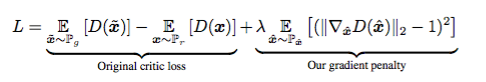
\includegraphics[width=1\textwidth]{penalty.png}
\end{figure}

\end{frame}

\begin{frame}
\frametitle{WGAN with gradient penalty}
\begin{figure}
\centering
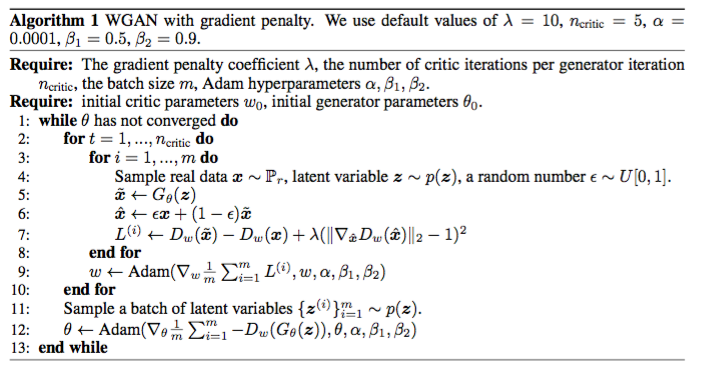
\includegraphics[width=1.07\textwidth]{i_wgan.png}
\end{figure}
\end{frame}

\end{document}